\chapter{Recurrent Neural Networks}
\label{ch:rnn}

\section{Introduction}

In the previous chapter, an argument was made for the use of models to for the purpose of anomaly detection. In this chapter, recurrent neural networks \cite{Rumelhart1986}, or RNNs, are introduced as powerful sequence modelers of arbitrary length.

RNNs have achieved state-of-the-art performance in supervised tasks such as handwriting recognition \cite{Graves2009}, and speech recognition  \cite{Graves2013}. RNNs can also be trained unsupervised to generate  music  \cite{Boulanger-Lewandowski2012}, text \cite{Martens2011a,Graves2013b}, and handwriting \cite{Graves2013b}. Given these impressive feats, RNNs can be effectively used for anomaly detection in sequences \cite{Marchi2015,Malhotra2015}.

Like HMMs, RNNs have hidden states. But, in contrast to HMMs, RNNs make a more efficient use of its hidden state \cite{ZacharyC.Lipton2015}. In a HMM, the hidden state depends only on the previous state which must store possible configurations of the sequence. So to incorporate information about an increasing window of previous states, the hidden state must grow exponentially large making them computationally impractical. While in RNNs, the state is shared over time; the hidden state of a RNN contains information from an arbitrarily long window. The next section will explain this.

In addition, RNNs do not make a Markovian assumption. In fact, they are so general, that RNNs have been shown to be equivalent to finite state automata \cite{Minsky1967}, equivalent to turing machines \cite{Siegelmann1995}, and more powerful than turing machines \cite{Siegelmann1993} even.

In the next few sections, some essential concepts of RNNs will be presented as most applicable to this work. Consult the RNN chapter in \cite{Bengio-et-al-2015-Book} for an in-depth treatment.

The precision from mathematical expressions will be used to understand how RNNs operate but only concepts will be presented. To follow the expressions precisely, some conventions are followed: 1) Due to the numerous interacting quantities, a typographic distinction is made between vectors ($\vc{v}$) and  matrices ($\mt{M}$). 2) Variables are time indexed with superscripts enclosed in parentheses ($\vc{x}^{(t)}$) leaving subscripts available to index other quantities.

% notation:
% matrix: bold upright 
% vector: italic bold
% funcs: 'normal' asis in mathmode.

\section{Recurrence}

Recurrence explains how a RNN stores a distributed state. Consider a dynamical system driven by signal $\vc{x}^{(t)}$ as in Equation \ref{eqn:ds}.

\begin{equation}
  \vc{s}^{(t)} = f(\vc{s}^{(t-1)},\vc{x}^{(t)};\vc{\theta})
  \label{eqn:ds}
\end{equation}

The state, $\vc{s}\tm{t}$, depends on the previous state, $\vc{s}^{(t-1)}$, through some function $f$ parameterized by $\vc{\theta}$. There is no restriction on the number of previous time steps. For example, for four previous time steps
\begin{equation*}
\vc{s}\tm{t} = 
f(f(f(f(\s\tm{t-4}
,\x\tm{t-3};\vc{\theta})
,\x\tm{t-2};\vc{\theta})
,\x\tm{t-1};\vc{\theta})
,\x\tm{t};\vc{\theta})     .
\end{equation*}

So the composite function, $g$, can be written as depending on an arbitrary number of time steps, $T$.
\begin{equation*}
\s\tm{T} = g_{T}(\x\tm{T},\x\tm{T-1},\x\tm{T-2},\ldots,\x\tm{2},\x\tm{1})
\end{equation*}
In other words, the vector $\s\tm{T}$ contains a summary of the of the preceding sequence, $(\x\tm{T},\x\tm{T-1},\x\tm{T-2},\ldots,\x\tm{2},\x\tm{1})$, through $g_T$.

It can be difficult to follow recurrent computations by looking at mathematical expressions. So recurrence can be graphically represented in two ways. One way, shown in Figure \ref{fig:recurrent}, shows the state feeding back into itself through its parameters representing Equation \ref{eqn:ds}. The other way is to `unfold' the recurrence in a flow graph as in Figure \ref{fig:recurrent_uf}. Graphs offer a convenient way of organizing computations. The (unfolded) graph shows every hidden state, say $\s\tm{t}$, is dependent on the current input, $\x\tm{t}$, the previous state, $\s\tm{t-1}$, and (fixed) parameters $\vc{\theta}$. So it should be obvious that $\vc{\theta}$ is shared over successive computations of $\s$.

\begin{figure}[H]
  \centering
  \begin{subfigure}[]{.2\textwidth}
    \begin{center}
    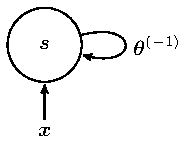
\includegraphics[]{figs/recurrent.pdf}
    \end{center}
    \caption{cyclic}
    \label{fig:recurrent}
  \end{subfigure}
  \begin{subfigure}[]{.79\textwidth}
    \begin{center}
    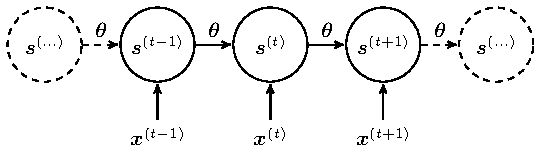
\includegraphics[]{figs/recurrent_uf.pdf}
    \end{center}
    \caption{acyclic (unfolded)}
    \label{fig:recurrent_uf}
  \end{subfigure}
  \caption{Recurrence Graph Views}
  \label{fig:recurrence}
\end{figure}


\section{Basic Recurrent Neural Network}

The functionality of a basic RNN resembles that of a traditional neural network with the addition of a state variable shared over time.


The core RNN functionality can be formulated as Equations \ref{eqn:rnn} describe. Each equation represents a `layer' or, individually, in the scalar sense, `nodes' in the network.
% no new para
\begin{subequations}  
  \label{eqn:rnn}
  \begin{align}
    \s\tm{t}&=
              \mathrm{\tanh}(
              \mt{W}_{ss}
              \s\tm{t-1}
              +
              \mt{W}_{xs}
              \x\tm{t}
              +
              \vc{b}_s
              ) 
              \label{eqn:rnns} \\ 
    \vc{o}\tm{t}&=
             \mt{W}_{so}
             \s\tm{t}
             +
             \vc{b}_{o}
             \label{eqn:rnno}
  \end{align}
\end{subequations}
\noindent 
The output at time $t$, $\vc{o}\tm{t}$, depends on current state, $\s\tm{t}$, which, in turn, depends on the previous state, $\s\tm{t-1}$, and the current input, $\x\tm{t}$, through associated weight matrices, $\mt{W}$. The weight matrices are subscripted with two variables to associate an input with an output. The input variable is the first subscript while the output variable is the second. For example, $\mt{W}_{so}$ connects the input from $\s$ to output, $\vc{o}$. Also, bias vectors, $\vc{b}$, allow values to be adjusted additively (offset). Finally, the hyperbolic tangent, $\tanh$, provides a non-linearity, in the range (-1,1), that allows the RNN to summarize arbitrarily complex sequences.

A `size' can be specified that measures the capacity of $\s$; the dimension of $\s$ is a (free) parameter (obviously the dimensions of other quantities in Equation \ref{eqn:rnns} need to be compatible).
%
No size is associated with $\vc{o}$ because it is restricted by the dimension of a given output, $\vc{y}$ (read further).

The output, $\vc{o}$, needs to be need to be compared to a `target', $\vc{y}$, through a loss function, $L$. For predicting sequences as targets, the mean squared error is a common choice for the loss function. Squared differences are summed and averaged over and the number of variables of the sequence resulting in a scalar as shown in Equation \ref{eqn:mse}.

\begin{equation}
  \label{eqn:mse}
  L(\vc{o},\vc{y}) = \frac{1}{TV} \sum_t \sum_v(
  \vc{o}\tm{t}_v - \vc{y}\tm{t}_v
  )^2,
\end{equation}
\noindent
$V$ and $T$ are the number of variables and the length of the sequences respectively indexed by $t$ and $v$ respectively.

Equations \ref{eqn:mse} and \ref{eqn:rnn}, together, define the framework for a basic RNN. One way to enhance this is to `stack' states so that the output from one state is input into another state in the same time step. So the last, $l$th, layer produces $\vc{o}$.  There is evidence that stacking the state layers leads to the network being able to learn time series at multiple time scales \cite{Hermans2013,Pascanu2013a}.


\begin{figure}[H]
  \centering
  \begin{subfigure}[]{.2\textwidth}
    \begin{center}
    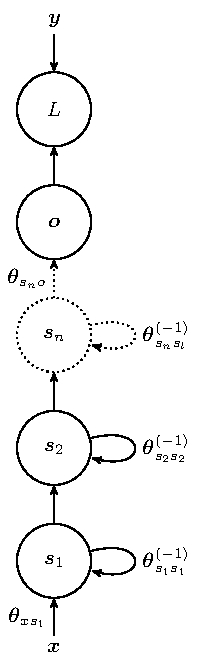
\includegraphics[]{figs/rnn.pdf}
    \end{center}
    \caption{cyclic}
    \label{fig:rnn_f}
  \end{subfigure}
  \begin{subfigure}[]{.79\textwidth}
    \begin{center}
    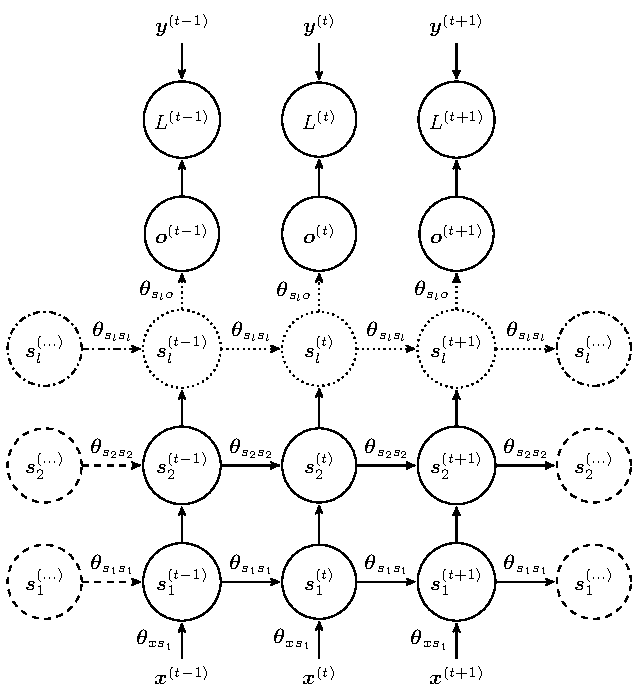
\includegraphics[]{figs/rnn_uf.pdf}
    \end{center}
    \caption{acyclic}
    \label{fig:rnn_uf}
  \end{subfigure}
  \caption[Recurrent neural network graph views]{
Recurrent neural network graph views. 
%this was all in the paragraph
Bias terms are omitted for clarity but are included as elements in $\vc{\theta}$ along with elements from $\W$.
%
The notation of $\vc{\theta}$ follows that of $\mt{W}$ but captures more variables by vectorizing each component for concatenation into a single vector.
%
$\vc{\theta}_{ss} = (\vc{W}_{ss},\vc{b}_s)$, $\vc{\theta}_{xs} = (\vc{W}_{xs})$, and $\vc{\theta}_{so} = (\vc{W}_{so},\vc{b}_o)$ (operations to produce the vector are implied).
%
Inter-layer parameters, $\vc{\theta}_{s_is_{i+1}}$, are omitted as well to focus on operations in time (horizontally).
}
  \label{fig:rnn}
\end{figure}%

The stacking can be seen graphically in Figure \ref{fig:rnn}. Notice that the unfolded view allows one to see that information can flow through many paths in time and layers (horizontally and vertically respectively). So `depth' can be used to describe the number of operations in these two directions with depth in the time direction being typically much greater\footnote{This makes RNNs, among `deep learning' architectures, the deepest networks!}.


\section{Training}

%use s_(l)ayers. todo

To train the network, the loss function is used to  minimize (optimize) an objective function given pairs of training examples, $(\x,\vc{y})$, by adjusting the parameters $\vc{\theta}$. Unfortunately, training neural networks in general, let alone recurrent neural networks, are challenging optimization and computational problems \cite{Blum1992}. However, a flavor of the relatively simple mini-batch stochastic gradient descent (SGD) has remained successful in training a variety of networks \cite{Bengio2012b} despite the availability of other, perhaps more sophisticated, optimization algorithms. %practical recs for training deep. todo 2014+ ref?

In plain mini-batch SGD, parameters are updated with a `learning rate', $\alpha$, for a selected `mini-batch' example set (from the training set), $M$, according to Equation \ref{eqn:sgd} until a convergence criterion is met.

\begin{equation}
  \label{eqn:sgd}
   \Delta \vc{\theta} =
   -\alpha
   \frac{1}{|M|} \sum_{(\vc{x}_m,\vc{y}_m) \in M}
   \frac{\partial{L}(
     \vc{o}%(\x_m;\vc{\theta})
     ,\vc{y}_m)}
   {\partial{\vc{\theta}}}
\end{equation}
%todo: make  summation bigger

Unfortunately, RNNs can suffer acutely from the vanishing (and exploding) gradient problem which makes learning long range dependencies difficult \cite{Hochreiter,Bengio1994,Doya1992,Pascanu2013c}.

The problem is understood through the calculation of $\partial{L}/\partial{\vc{W}_{ss}}$ for a `history' of $T$ points prior to $t$.
%
An involved application of the (backpropagated) differential chain rule to the loss function using the \emph{basic} (unfolded) RNN defined in Equations \ref{eqn:rnn} leads to Equation \ref{eqn:grad}.

\begin{equation}
  \label{eqn:grad}
  \frac{\partial{L}\tm{t}}{\partial{\vc{W}_{ss}}} = 
  \sum_{i=0}^T
  \frac{\partial{    L}\tm{ t}}{\partial{\vc{o}\tm{t}}}
  \frac{\partial{\vc{o}}\tm{t}}{\partial{\vc{s}\tm{t}}}
  \left(
    \prod_{j=i+1}^{T}
    \frac{\partial{\vc{s}}\tm{j}}{\partial{\vc{s}\tm{j-1}}}
  \right)
  \frac{\partial{\vc{s}}\tm{i}}{\partial{\vc{W}_{ss}}}
\end{equation}
%
\noindent
Equation \ref{eqn:grad} shows that there are multiplicative `chains' of differentials for each preceding time step. 

\begin{figure}[H]
  \centering
  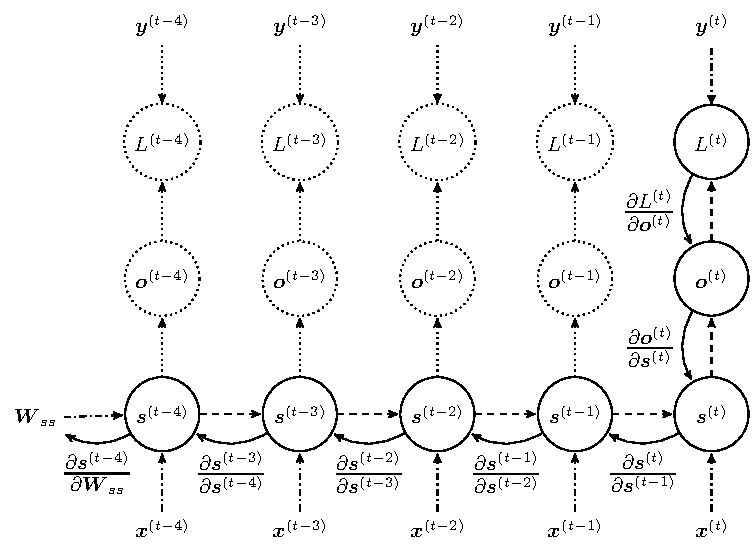
\includegraphics[]{figs/grad.pdf}
  \caption[Partial derivative chain for a basic RNN]{Partial derivative chain for a basic RNN for a history of 4 time steps (biases not shown).
%this used to be in the paragraph.
%
Several quantities are distinguished. Dash-dotted lines are the independent inputs, $\x$, $\vc{y}$, and $\vc{W}_{ss}$, to the loss function, $L$, while the dashed lines represent intermediate quantities in the graph.
%
The path formed by the curved solid lines follows the chain rule to get one summand for $\partial{L}\tm{t}/\partial{\vc{W}_{ss}}$.
%
Dotted quantities are not involved in the calculation (for $T=4$).

}
  \label{fig:grad}
\end{figure}

The computational graph in Figure \ref{fig:grad} represents Equation \ref{eqn:grad} for $T=4$.
%
Now that the graph is associated with the equation, the origin of the vanishing gradient can be seen;
%
the vanishing gradient is due to successive multiplications of the derivative of $\tanh$ which is bound in $(0,1]$ (Again, see \cite{Hochreiter,Bengio1994,Doya1992,Pascanu2013c} for details).


\cite{Bengio-et-al-2015-Book} (sec. 10.7) lists ways in which the problem can be mitigated by applying different RNN architectures or enhancing the optimization process.
%
For example, Hessian-free optimization \cite{Martens2010} uses second order information that can make use of the ratio of small gradients to small curvature to more directly find optimal parameters.
%
\cite{Martens2011} uses Hessian-free optimization to train a basic RNN to achieve remarkable results.
%
However, this comes at a computational cost.
%
For practical reasons, it might be preferable to use well-established SGD-based methods over second order methods \cite{Bengio2012,Dauphin} as long as the RNN architecture facilitates learning long range dependencies;
%
the Long Short Term Memory (LSTM) RNN \cite{Hochreiter1997} uses a `memory cell' to recall (past) information only when needed thereby working around the vanishing gradient problem.




\section{Long Short-Term Memory} %todo check hyphenations

LSTM models have achieved impressive benchmarks recently.
%
Networks with LSTM elements have been used for
text-to-speech synthesis \cite{Fan2014},
language identification from speech \cite{Gonzalez-Dominguez2014},
large-vocabulary speech recognition \cite{Sak2014},
English-to-French text translation  \cite{Sutskever2014},
identifying non-verbal cues from speech \cite{Brueckner2014},
Arabic handwriting recognition \cite{Bluche},
image caption generation \cite{Vinyals2015},
video to text description \cite{Venugopalan2014},
and generating realistic talking heads \cite{Fan2015}.
%
Furthermore, LSTM RNNs have remained competitive against other RNN types \cite{Jozefowicz2015}.


There are a few variants of LSTM but they all have a linear self-loop that gradients can flow through for a long time.
%
LSTM variants have not shown to differ greatly in performance \cite{Greff2015}.
%
The equations describing the LSTM state involve significantly more steps than the basic RNN state equation, Equation \ref{eqn:rnn}.
%
So, the mathematical procedure for the LSTM state is presented with a figure.
%
The LSTM variant presented in Figure \ref{fig:lstmfig} is found in \cite{Graves2013b}.

\begin{figure}[H]
  \centering
  \begin{subfigure}[]{\textwidth}
    \begin{center}
    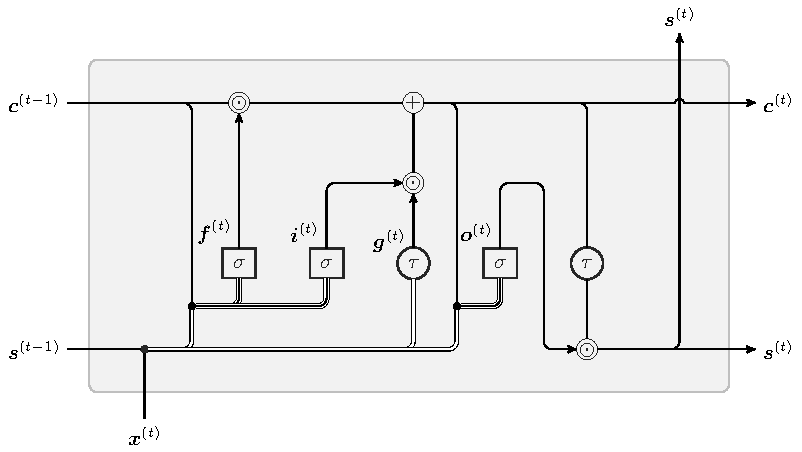
\includegraphics[]{figs/lstm.pdf}
    \end{center}
    \caption{calculation flow diagram (biases omitted, inspired by \cite{Colah2015})}
    \label{fig:lstm} 
  \end{subfigure}
  \begin{subfigure}[]{\textwidth}
    \begin{subequations}
      \begin{align}
        \vc{i}\tm{t} 
        &= 
          \sigma
          (
          \mt{W}_i \cdot
          (
          \x\tm{t},
          \vc{s}\tm{t-1},
          \vc{c}\tm{t-1}
          )
          +\vc{b}_i
          ) 
        \\
        \vc{f}\tm{t} 
        &=
          \sigma
          (
          \mt{W}_f \cdot
          (
          \x\tm{t},
          \vc{s}\tm{t-1},
          \vc{c}\tm{t-1}
          )
          +\vc{b}_f
          )
        \\
        \vc{g}\tm{t}
        &=
          \tanh
          (
          \mt{W}_c \cdot
          (
          \x\tm{t},
          \vc{s}\tm{t-1}
          )
          +\vc{b}_c
          )
        \\
        \vc{c}\tm{t} 
        &= 
          \vc{f}\tm{t}   \odot \vc{c}\tm{t-1}
          + \vc{i}\tm{t} \odot \vc{g}\tm{t}
        \label{eqn:lstms}\\
        \vc{o}\tm{t}
        &=
          \sigma
          (
          \mt{W}_o \cdot
          (
          \x\tm{t},
          \vc{s}\tm{t-1},
          \vc{c}\tm{t-1}
          )
          +\vc{b}_o
          )
        \\
        \vc{s}\tm{t}
        &=
          \vc{o}\tm{t} \odot
          \tanh
          (
          \vc{c}\tm{t}
          )
      \end{align}
    \end{subequations}
    \caption{equations from \cite{Graves2013b}}
    \label{eqn:lstm}
  \end{subfigure}
  \caption{Long Short-Term Memory Layer.
%
$\sigma$ stands for the logistic sigmoid function while $\tau$ stands for $\tanh$.
%
Element-wise multiplication is represented by the $\odot$ symbol.
%
For brevity and clarity, a (single) weight matrix combines the weights associated with more than one input to a single output (unlike the typical notation used in literature).
%
For example, $\mt{W}_i \cdot(\x\tm{t},\vc{s}\tm{t-1},\vc{c}\tm{t-1})=\mt{W}_{xi}\vc{x}\tm{t}+\mt{W}_{si}\vc{s}\tm{t-1}+\mt{W}_{ci}\vc{c}\tm{t-1}$ where the input vectors, $\x$, $\vc{s}$, and $\vc{c}$ are concatenated into a vector  and weight matrices $\mt{W}_{xi}$, $\mt{W}_{si}$, and $\mt{W}_{ci}$ are augmented horizontally. %todo.. chk dim in theanets code
%
In the diagram, the concatenation is represented by black dots combining single lines into more than one line.
%
Furthermore, $\mt{W}_{ci}$, $\mt{W}_{cf}$, and $\mt{W}_{co}$ are diagonal matrices so the number of weights associated with each $\vc{c}$ equals the LSTM `size'.
}
  \label{fig:lstmfig}
\end{figure}


The size that can be attributed to the LSTM module is the dimension of $\vc{i}$, $\vc{f}$, $\vc{g}$, $\vc{c}$, $\vc{o}$, or $\vc{s}$ (which are equal).


Very briefly, the central element in a LSTM module is the `memory cell', $\vc{c}$, that works to keep information unchanged over many time steps (likened to a conveyor belt through time).
%
Information flow is controlled through input, `forget', and output `gates', elements $\vc{i}$, $\vc{f}$, and $\vc{o}$ respectively.
%
The input gate controls information into the memory cell.
%
The output gate controls when information should flow to the next time step.
%
The forget gate zeros out elements in the memory cell.
%
The gates make their decisions based on the input, $\x$, the `hidden' state, $\vc{s}$, and content already in the memory cell.
%
%g is a c candidate
%things get trapped in memory

%c has stuff nominally 0-1 while h has -1,1 behaves more like regular rnn
% how c 0,1 if g can be -1,1
% i can imagine if c had a 1. there would be a way for it to stay
%things could be simpler in alt. to LSTMS!
%original lstm paper to know whys of everything

% The following enumeration conceptually outlines the operation of the LSTM module.

% \begin{enumerate}
% \item[1. ] sfd
% \end{enumerate}

% proc
% 1
% 2
% 3

% math that shows lstm gets around vanishing grad

Unlike the recurrence of the basic RNN (Equation \ref{eqn:rnns}), information can be kept for a long time in the recurrence chain of $\vc{c}$ (Equation \ref{eqn:lstms}). 
%
There is a way for information to propagate without successive multiplication of fractions (as in the derivative of $\tanh$):
%
In Equation \ref{eqn:lstms}, consider an element in (vector) $\vc{c}\tm{t-1}$ with a value of 1.
%
It can be retained indefinitely as long as the corresponding element in $\vc{f}\tm{t}$ is 1 and the corresponding element in $\vc{i}\tm{t}$ is 0.
%
In other words, the derivative is constant with respect to $t$.

Finally, note how the LSTM modules can be stacked (vertically) in similar fashion to the basic RNN.
%
The output of the lower module, $\vc{s}\tm{t}$, becomes the input, $\x\tm{t}$, of the upper module.


With such configurations, the next chapter will show how LSTM RNNs can be used to model time series to find anomalies.

% lstm:
% CECs are
% the main reason why LSTM nets can learn to discover the importance of (and memorize) events that
% happened thousands of discrete time steps ago, while previous RNNs already failed in case of minimal
% time lags of 10 steps


%%% Local Variables:
%%% mode: latex
%%% TeX-master: "thesis"
%%% End:
